% THIS IS AN EXAMPLE DOCUMENT FOR VLDB 2012
% based on ACM SIGPROC-SP.TEX VERSION 2.7
% Modified by  Gerald Weber <gerald@cs.auckland.ac.nz>
% Removed the requirement to include *bbl file in here. (AhmetSacan, Sep2012)
% Fixed the equation on page 3 to prevent line overflow. (AhmetSacan, Sep2012)

\documentclass{vldb}
\usepackage{times}
\usepackage{graphicx}
\usepackage{balance}  % for  \balance command ON LASMAD PAGE  (only there!)
\usepackage{alltt,algo}
\usepackage{url}

\begin{document}

% ****************** TITLE ****************************************

\title{Introducing MADlib\\{\Large (MAD Skills, the SQL)}}


\numberofauthors{11} %  in this sample file, there are a *total*
% of EIGHT authors. SIX appear on the 'first-page' (for formatting
% reasons) and the remaining two appear in the \additionalauthors section.

\author{Joseph M. Hellerstein\\{\small U.C. Berkeley} \and
 Christoper Re\\{\small U. Wisconsin} \and
 Daisy Zhe Wang\\{\small U. Florida} \and
 Eugene Fratkin\\{\small Greenplum} \and
 Aleks Gorajek\\{\small Greenplum} \and
 Steven Hillion\\{\small Alpine Data Labs} \and
 Luke Lonergan\\{\small Greenplum} \and
 Kee Siong Ng\\{\small Greenplum} \and
 Florian Schoppmann\\{\small Greenplum} \and
 Gavin Sherry\\{\small Greenplum} \and
 Caleb Welton\\{\small Greenplum}}

\maketitle

\begin{abstract}
  MADlib is a free, open-source library of in-database analytic methods.
  It provides an evolving suite of SQL-based algorithms for machine
  learning, data mining and statistics that run at scale within a
  database engine, with no need for data import/export to other tools.
  The goal is for MADlib to eventually serve a role for scalable
  database systems that is similar to the CRAN library for R: a
  community repository of statistical methods, this time written with
  scale and parallelism in mind.

  In this paper we introduce the MADlib project, including the
  background that led to its beginnings, and the motivation for its
  open-source nature.  We provide an overview of the library's
  architecture and design patterns, and provide a detailed description
  of one example method in that context.  We then report on initial 
  efforts incorporating academic research into MADlib, which is one of the 
  project's goals. Finally, we report on early
  performance results in the open-source PostgreSQL DBMS, and scaling
  results in the Greenplum parallel DBMS.  
  
  MADlib is freely
  available in beta form at http://madlib.net, and the project is open
  for contributions of both new methods, and ports to additional
  database platforms.  
\end{abstract}




\section{Introduction:\\From Warehousing to Science}
\noindent
Until fairly recently, large databases were used mainly for accounting
purposes in enterprises, supporting financial record-keeping,
reporting and analysis at various levels of granularity.  {\em Data
Warehousing} was the name given to industry practices for these
database workloads.  Accounting, by definition, involves significant
care and attention to detail. Data Warehousing practices followed suit
by encouraging careful and comprehensive database design, and by following exacting policies regarding the quality of data loaded into the database.

Attitudes toward large databases have been changing quickly in the
past decade, as the focus of large database usage has shifted from
accountancy to analytics.  The need for correct accounting and data
warehousing practice has not gone away, but it is a becoming a
shrinking fraction of the volume---and the value---of large-scale data
management.  The emerging trend focuses on the use of a wide range of
potentially noisy data to support predictive analytics, managed by
statistical models and algorithms for analysis.  {\em Data Science} is a
name that is gaining currency for the industry practices evolving
around these workloads.

Data scientists make use of database engines in a very different way than traditional data warehousing professionals.  Rather than carefully
designing global schemas and ``repelling'' data until it is integrated,
they load data into private schemas in whatever form is convenient.  Rather than focusing on simple OLAP-style drill-down reports, they implement rich statistical
models and algorithms in the database, using extensible SQL as a
language for orchestrating data movement between disk, memory, and multiple parallel machines.  In short, for data scientists a DBMS is a scalable analytics runtime---one that is conveniently compatible with the database systems widely used for transactions and accounting.

In 2008, a group of us from the database industry, consultancy,
academia, and end-user analytics got together to describe this usage
pattern as we observed it in the field.  We dubbed it {\bf MAD}, an acronym for the {\em Magnetic} (as opposed to
repellent) aspect of the platform, the {\em Agile} design patterns used for
modeling, loading and iterating on data, and the {\em Deep} statistical models and
algorithms being used.  The ``MAD Skills'' paper that resulted described
this pattern, and included a number of non-trivial analytics
techniques implemented as simple SQL scripts~\cite{madskills}.

After the publication of the paper, it became clear that there was
significant interest not only in its design aspects, but
also in the actual SQL implementations of statistical methods.  This
interest came from every constituency involved: customers were
requesting it of consultants and vendors, and academics were
increasingly publishing papers on the topic.  What was missing was a
software framework to focus the energy of the community, and connect
the various interested constituencies.  This led to the design of
{\bf MADlib}, the subject of this paper.  

\subsection*{Introducing MADlib}
MADlib is a library of analytic methods that can be installed and
executed within a relational database engine that supports extensible
SQL.  A snapshot of the current contents of MADlib including methods and
ports is provided in Table~\ref{tab:methods} and Table~\ref{tab:ports}.  This set of methods and ports is intended to grow over time.

The methods in MADLib are designed for the shared-nothing, ``scale-out''
parallelism offered by modern parallel database engines, ensuring that
computation is done close to the data.  The core functionality is
written in declarative SQL statements, which orchestrate massively
parallel data movement.  Single-node inner loops take advantage of SQL
extensibility to call out to high-performance math libraries in
user-defined scalar and aggregate functions.  At the highest level,
tasks that require iteration and/or structure definition are coded in
Python driver code, which is used only to kick off the data-rich
computations that happen within the parallel database engine.

MADlib is hosted publicly at github, and readers are encouraged to
browse the code and documentation via the MADlib website
\url{http://madlib.net}.  The initial MADlib codebase reflects contributions
from both industry (Greenplum) and academia (UC Berkeley, the
University of Wisconsin, and the University of Florida).  Code
management and Quality Assurance efforts have been contributed by
Greenplum.  At this time, the project has begun welcoming
contributions from additional parties, including both new methods and
ports to new platforms.

\begin{table}
  \begin{tabular}{|l|l|}
    \hline
    {\bf Category} & {\bf Method} \\ \hline\hline
    Supervised Learning
          & Linear Regression\\
          & Logistic Regression \\
          & Naive Bayes Classification\\
          & Decision Trees (C4.5)\\
          & Support Vector Machines\\ \hline
    Unsupervised Learning
          & k-Means Clustering\\
          & SVD Matrix Factorization\\
          & Latent Dirichlet Allocation\\
          & Association Rules\\ \hline
    Decriptive Statistics
          & Count-Min Sketch\\
          & Flajolet-Martin Sketch\\
          & Data Profiling\\
          & Quantiles\\ \hline
    Support Modules
          & Sparse Vectors\\
          & Array Operations\\
          & Conjugate Gradiant Optimization \\\hline
  \end{tabular}
\caption{Current MADlib methods.  (We may want to rate these with markers for maturity.  Also have to decide what to include here from UW and UF.)}
\label{tab:methods}
\end{table}

\begin{table*} 
  \begin{center}
  \begin{tabular}{|p{1.25in}|p{1.75in}|p{3.5in}|}
  \hline
  {\bf DBMS} & {\bf R\&D Access} & {\bf Notes}\\ \hline
    PostgreSQL& Open source & Single-node only. \\ \hline
    Greenplum Database & ``Community Edition'' available free for non-production use & Shared-nothing parallel DBMS for clusters and multicore. \\ \hline
     \end{tabular}
\end{center}
\caption{Current MADlib ports.}
\label{tab:ports}
\end{table*}

\section{Goals of the Project} 
The primary goal of the MADlib open-source project is to accelerate
innovation and technology transfer in the Data Science community via a shared
library of scalable in-database analytics, much as the CRAN library
serves the statistics community~\cite{cran}.  Unlike CRAN, which is
customized to the R analytics engine, we hope that MADlib's grounding
in standard SQL will lead to community ports to a
variety of parallel database engines.

In addition to its primary goal, MADlib can serve a number of other
purposes for the community.  As a standard and relatively mature
open-source platform, it enables apples-to-apples comparisons that can
be deeper than the traditional TPC benchmarks. For example, the DBMS
backend can be held constant, so that two algorithms for the same task
(e.g., entity extraction) can be compared for runtime and answer
quality.  Similarly, as MADlib is ported to more platforms, an
algorithm can be held constant, and two backend DBMS engines can be
compared for performance.  This latter comparison has been notoriously
difficult in the past, due to the closed-source, black-box nature of
``data mining'' and analytic toolkits that were not only customized to
specific platforms, but also lacked transparency into their analytic
algorithms.  

\subsection{Why Databases?}

For decades, statistical packages like SAS, Matlab and R have been the key tools for deep analytics, and the practices surrounding these tools have been elevated into widely-used traditional methodologies.  
% DELETED -- better not to pick fights with specific vendors.  -JMH
% SAS in particular has a
% large customer base, and its proposed analytics methodologies have
% become engrained in the modern enterprise. Nevertheless, usurpers loom
% on the horizon. 
One standard analytics methodology advocated in this domain
is called SEMMA: Sample, Explore, Modify, Model, Assess. The ``EMMA''
portion of this cycle identifies a set of fundamental tasks
that an analyst needs to perform, but the first, ``S'' step makes less and less sense in many settings today.  The costs of computation and storage are increasingly cheap, and entire data sets can often be processed efficiently by a cluster of computers.  Meanwhile, competition for extracting value from data has become increasingly refined.  Consider fiercely competitive application domains like online advertising or politics.  It is of course important to target ``typical'' people (customers, voters) that would be captured by sampling the database.  Because SEMMA is standard practice, optimizing for a sample provides no real advantage.  The competition today is to extract advantages in the long tail of ``special interests'', a practice known as ``microtargeting'', ``hypertargeting'' or ``narrowcasting''.  In that context, the first step of SEMMA essentially defeats the remaining four steps, leading to simplistic, generalized decision-making that may not translate well to small populations in the tail of the distribution.
% throws away the very
% competitive advantage that customers hope to get from acquiring their
% valuable data. Sampling decouples the human intelligence in
% modeling from where these insights are put to use (on the entire
% data). This decoupling makes analysts less effective: they must guess
% about the statistical and performance robustness of their model. If
% they guess incorrectly, they may not know about it for weeks or
% months. (SAID BETTER BY PEOPLE WHO TALK GET TO REGULARLY TALK TO
% CUSTOMERS)

Driven in part by this observation, momentum has been gathering around efforts to develop scalable full-dataset analytics. One popular alternative is to
push the statistical methods directly into so-called Big Data processing platforms---notably, Apache Hadoop. For example, the open-source Mahout project
aims to implement machine learning tools within Hadoop, harnessing
 interest in both academia and industry~\cite{mlformr,mahout}. This is
certainly an attractive path to solution, and is being advocated by
major players including IBM~\cite{}.

At the same time that the Hadoop ecosystem has been evolving, the SQL-based analytics ecosystem has grown rapidly as well, and large volumes of valuable data are likely to reside in
relational databases for many years to come. There is a rich
ecosystem of tools, know-how, and organizational requirements that
encourage this.  For these cases, it would be helpful to push statistical methods into the DBMS. And as we will see, massively parallel databases form a surprisingly useful platform for sophisticated analytics.  MADLib currently targets this environment of in-database analytics.

%% There is nothing to be gained by pissing on Hadoop.  -- JMH
% there
% are drawbacks with the Hadoop approach: its performance is untenably
% slow compared to database processing as it must provide higher levels
% of fault tolerance than other systems. Additionally, the sheer number
% of machines that are required to achieve good performance of makes it
% unclear that Hadoop systems are cost-effect in all but the most scale
% heavy environments.
% 
% For such users, Greenplum provides a cost-effective solution for
% scalable analytics. It does not require a complicated and error-prone
% import/export cycle to Haddop nor forces the user to work over a
% snapshot of the data: one works on the raw data and does their
% analysis on production (or very near-to-production) data. This allows
% user to maximize the value proposition of storing all that data in a
% cost-effective manner.

%%   Q1: why not SAS?  Q2: what about the fact that SQL nerds don�t do
%%   data analysis?  Q3: does Hadoop and Mahout make this irrelevant?

%% Chris asked Q1 and Q2 this way:

%% There is another major shift that MADLib potentially allows:
%%   analysts can get closer to their data than ever before. For
%%   example, SAS promotes a model of an analysts workflow called SEMMA
%%   model (Sample, Explore, Modify, Model, Assess). This is (afaik) the
%%   industry standard. To me, what's totally busted about this loop is
%%   the S -- if you're looking for something rare, the sampling step
%%   throws out the most interesting bits! Then your EMM steps where you
%%   build understanding are of a small fraction of your data. This is
%%   the part where the analyst is currently far from the data. As a
%%   result, their entire conversation is not with the data but with a
%%   small sample. If something goes wrong, you (maybe) find out about
%%   it in the A step (which is on the whole data).

%%   Moreover, it's totally unnecessary to do the S loop in the MADLib
%%   world view, and the fact that the S step has been elevated to the
%%   level of feature is a testament to how broken the current tool
%%   chain is.
%% A couple follow-on points:

%%     * WRT SAS and sampling, the way I heard it from the FAN guys it�s all about competitive advantage in the tails of the distribution.  Something like �anybody can tackle the 20% of cases in the head of the distribution.  The competitive advantage is in tackling the long tails: e.g. target ads to toyota-truck-driving-latin-music-loving-sushi-eating women in cold climates.�  Simple sample/extract techniques blow on that stuff.
%%     * WRT Hadoop/Mahout:  I think we need to mention it here and acknowledge it�s been an attractive path to a solution, and Hadoop certainly is getting the attention of the Web and ML communities [Stanford paper].  Mahout is an attempt to package that energy, with some institutional support from MapR.  But despite the success of MapReduce, lots of important data is still going into databases and will continue to do so for years to come for a host of reasons that are both technical and organizational.  Even if Mahout succeeds wildly (and it isn�t doing so to date, but I don�t think we want to bother saying that), there�s a critical vacuum to be filled in SQL-land.  What we can (re-)learn from the Hadoop community is the power of open-source teamwork, and the desire for agile platforms for analytics.  There�s no reason we can�t direct that agile thinking toward the data in databases.
%% *


\subsection{Why Open Source?}


From the beginning, MADlib was designed as an open source project with
corporate backing, rather than a closed-source corporate effort with
academic consulting.  This decision was motivated by a number of
factors, including the following:

\begin{itemize}
    \item \textbf{The benefits of customization}: Statistical methods are rarely used as turnkey solutions.  As a result, it is common for data scientists to want to modify and adapt canonical models and methods (e.g., regression, classification, clustering) to their own purposes.  This is a very tangible benefit of open source libraries over traditional closed-source packages. Moreover, in an open-source community there is a process and a set of positive incentives for useful modifications to be shared back to the benefit of the entire community.
    \item \textbf{Valuable data vs.\ valuable software}:  In many emerging business sectors, the corporate value is captured in the data itself, not in the software used to analyze that data.  Indeed, it is in the interest of these companies to have the open-source community adopt and improve their software.  Open-source efforts can also be synergistic for vendors that sell commercial software to customers who run open-source code.  Most IT shops today run a mix of open-source and proprietary software, and it is wise for software vendors to position themselves intelligently in that context.  For many database system vendors, their core competency is not in statistical methods, but rather in the engines that support those methods, and the service industry that evolves around them.
    \item \textbf{Closing the research-to-adoption loop}:  Very few companies that depend on data analysis have the capacity to develop significant in-house research into computing or data science.  On the other hand, it is hard for academics doing computing research to understand and influence the way that analytic processes are done in the field.  An open source project like MADlib has the potential to connect academic researchers not only to industrial software vendors, but also directly to the end-users of analytics software.  This can improve technology transfer from academia into practice without requiring database software vendors to serve as middlemen.  It can similarly enable end-users in specific application domains to influence the research agenda in academia.
    \item \textbf{Leveling the playing field, encouraging innovation}:  Over the past two decades, database software vendors have developed proprietary data mining toolkits consisting of textbook algorithms.  It is hard to assess their relative merits.  Meanwhile, other communities in machine learning and internet advertising have also been busily innovating, but their code is typically not well packaged for reuse, and the code that is available was not written to run in a database system.  Meanwhile, none of these projects has demonstrated the vibrancy and breadth we see in the open-source community surrounding R and its CRAN package.  A robust open-source project like MADlib can bring the entire database community up to a baseline level of competence on standard statistical algorithms, remove the corporate \textit{FUD}  from proprietary toolkits that has held back innovation, and help focus a large community on innovation and technology transfer.
\end{itemize}

\subsection{A Model for Open Source Collaboration}

The design of MADlib comes at a time when the connections between
open-source software and academic research seem particularly frayed.
MADlib is designed in part as an experiment in binding these
communities more tightly, to face current realities in software
development.

In previous decades, open-source software famously came from universities and evolved into significant commercial products.  Examples include the Ingres and Postgres database systems, the BSD UNIX and Mach operating systems, the X-windows user interfaces and the Kerberos authentication suite.  These projects were characterized by aggressive application of cutting-edge research ideas, captured in workable but fairly raw public releases that matured slowly with the help of communities outside the university.  While all of the above examples were incorporated into commercial products, many of those efforts emerged years after the initial open-source releases, and often with significant changes.

Today, we expect successful open source projects to be quite mature,
often comparable to commercial products.  To achieve this level of
maturity, most successful open-source projects have one or more major
corporate backers who pay some number of committers and provide
professional support for Quality Assurance (QA).  This kind of investment is typically
made in familiar software packages that tend not to feature new
research ideas.  Many of the most popular examples---Hadoop, Linux,
OpenOffice---are direct clones of well-identified,
pre-existing commercial efforts.

MADlib is making an explicit effort to back up academic research with professional software engineering.  Many academic research projects are supported by financial grants and gifts from companies.  In MADlib, the corporate donation consists of significant work hours from professional software engineers.  This leverages a strength of industry that cannot be replicated on a university
campus.  Companies can hire high-quality, experienced software
engineers with the attraction of well-compensated, long-term career
paths.  Equally important, software shops can offer an entire software
engineering pipeline that cannot be replicated on campus:
this includes QA processes encompassing specialized QA engineers as
well as software testing procedures and hardware platforms for
automated testing at scale.  The hope is that the corporate staffing of research projects like MADlib can both enable
academic open-source research, and speed technology transfer to industry.
\subsection{Status and Directions for Growth}

The initial beta release of MADlib in {\bf MONTH} of 2012 was focused on establishing a baseline of 
valuable functionality, while laying the groundwork for future evolution.  The beta development began with the non-trivial work of building the general-purpose
framework described in Section~\ref{sec:gen}.  Additionally, we wanted robust
implementations of textbook methods that were most frequently
requested from customers we met through Greenplum.  Finally, we wanted
to validate MADlib as a research vehicle, by fostering a small number of  university groups working in the area to experiment with the platform and get their code disseminated.

% Discuss the initial selection of methods.  



With the recent MADlib release completed, there is room for growth in multiple
dimensions.  The library infrastructure itself is still in beta, and
has room to mature.  There is room for enhancements in its core
treatment of mathematical kernels (e.g.\ linear algebra over both
sparse and dense matrices) especially in out-of-core settings.  And of
course there will always be an appetite for additional statistical models and
algorithmic methods, both textbook techniques and cutting-edge research.  Finally,
there is nascent interest on the MADlib newsgroup in ports to other DBMSs. Porting MADlib across DBMSs is a
mechanical but non-trivial software development effort that will
span the infrastructure (e.g.\ the need for a cross-platform
installer), the methods themselves (particularly the user-defined
functions) and the software engineering infrastructure (e.g.\ the need
for QA support on additional database engines).

\section{MADlib Architecture}
\label{sec:gen}
The core of traditional SQL---\texttt{SELECT...} \texttt{FROM...} \texttt{WHERE}... \texttt{GROUP BY}---is
quite a powerful harness for orchestrating bulk data processing across
one or many processors and disks.  It is also a portable, native
language supported by range of widely-deployed open source and
commercial database engines.  This makes SQL an attractive
framework for writing data-intensive programs.  Ideally, we would like
MADlib methods to be written entirely in straightforward and portable
SQL. Unfortunately, the portable core of ``vanilla'' SQL is often not
quite enough to express the kinds of algorithms needed for advanced
analytics.

Many statistical methods boil down to linear algebra expressions over
matrices.  For relational databases to operate over very large
matrices, this presents challenges at two scales.  At a macroscopic
scale, the matrices must be intelligently partitioned into chunks that
can fit in memory on a single node.  Once partitioned, the pieces can
be keyed in such a way that SQL constructs can be used to orchestrate
the movement of these chunks in and out of memory across one or more
machines.  At a microscopic scale, the database engine must invoke
efficient linear algebra routines on the pieces of data it gets in
core.  To this end it has to have the ability to very quickly invoke
well-tuned linear algebra methods.

We proceed to discuss issues involved at both of these levels in a bit more detail, and solutions we chose to implement in MADlib.
\subsection{Macro-Programming (Orchestration)}

A scalable method for linear algebra depends upon divide-and-conquer techniques: intelligent
partitioning of the matrix, and a pattern to process the pieces and
merge results back together.  This partitioning and dataflow is
currently outside the scope of a traditional query optimizer or
database design tool.  But there is a rich literature from scientific
computing on these issues~\cite{demmel} that database programmers can use to craft efficient in-database implementations.  Once data is properly partitioned, database engines shine at orchestrating the
resulting data movement of partitions and the piecewise results of
computation.

In designing the high-level orchestration of data movement for analytics, we ran across two main
limitations in standard SQL which we describe next.  We addressed both limitations using driver code written in simple
script-based user-defined functions (UDFs), which in turn kick off more
involved SQL queries.  When implemented correctly, the performance of the scripting language code is not critical, since its logic is invoked only
occasionally to kick off much larger bulk tasks that are executed by
the core database engine.

The first problem we faced is a limitation of SQL's roots in
first-order logic, which requires that queries be cognizant of the
schema of their input tables, and produce output tables with a fixed
schema.  In many cases we want to write ``templated'' queries that
work over arbitrary schemas, with the details of column names and
types to be filled in later.  For example, the multivariate linear
regression algorithm of Section~\ref{sec:regression} is designed to run over any subset
of the columns of an input table, producing an output table including
the same columns as well as a predicted output column.  SQL helps with
problems of data types and casting, but cannot help with the variable
arity of inputs and outputs.  To address this issue, we use Python
UDFs to interrogate the database catalog for details of input tables,
and then synthesize customized SQL queries based on templates to
produce outputs.  {\bf Figure~\ref{fig:secondorder} shows Python code that illustrates this.} This pattern is currently done in an ad hoc way in
each method that needs it.  In future we plan to support this pattern
as a Python library that ships with MADlib.

A second problem is the prevalence of iterative algorithms for many
methods in statistics, particularly stochastic methods like Gradiant
Descent and Monte Carlo simulation in which the number of iterations
is determined by a data-dependent stopping condition at the end of
each round.  There are multiple SQL-based workarounds for this
problem, which depend on the context.  In order to drive independent
iterations, it is often simplest (and very efficient) to use a
set-oriented join---this is an approach that we used to implement
Bootstrap sampling in the original MAD Skills paper~\cite{MADSkills}.  For
settings where the current iteration depends on previous iterations,
SQL's windowed aggregate feature can sometimes work.   Wang, et al. took
this approach to implement in-database MCMC inference~\cite{Daisy11}.  Most
generally, it is possible to use the recursion features of SQL to
perform iteration with arbitrary stopping conditions---this was used by
Wang, et al.\ to implement Viterbi inference~\cite{Daisy10}.  Unfortunately,
the level of support for SQL's windowed aggregates and recursion
varies across database products, and does not form a reliable
basis for portability.

As a result, in MADlib we typically implement iterative methods by
writing a driver UDF in Python to control the iteration.  A standard
pitfall in this style of programming is to pull a large amount of data
out of the database and into the driver code; this becomes a
scalability bottleneck since the driver code typically does not
parallelize and hence pulls all data to a single node.  We avoid this
via a design pattern in which the driver UDF kicks off each iteration
and stages its output into a temporary table via \texttt{CREATE TEMP TABLE
AS SELECT...} It then interrogates the resulting temp table using small
aggregate queries as needed.  As a result, all large-data movement is
done within the database engine and its buffer pool.
Database engines typically provide efficient parallelism as well as
buffering and spill files on disk for large temp tables, so this
pattern is quite efficient in practice.
\subsection{MicroProgramming: Data Representations and Inner Loops}

In addition to doing the coarse-grained orchestration of chunks, the
database engine must very efficiently invoke the single-node code that
performs arithmetic on those chunks.  For dense matrices, the standard
practice is to write UDFs in C or C++ that use the database engine to
make native calls to an open-source library like LAPACK.  Sparse
matrices are not as well-handled by standard math libraries, and require
more customization for efficient representations both on disk and in
memory.  We chose to write our own sparse matrix library in C for
MADlib, which {\bf XXX SAY SOMETHING ABOUT THE REPRESENTATION}.  Both of
these solutions require careful low-level coding, and formed part of
the overhead of getting MADlib started.

The specifics of a given method's linear algebra can be coded in a
low-level way using loops of basic arithmetic in a language like C,
but it is nicer if they can be expressed in a higher-level syntax that
captures the semantics of the linear algebra at the level of matrices
and arrays.  We provide a C++ abstraction layer in MADlib for this
type of code.  

\subsection{Example: Linear Regression Background}

\begin{itemize}
    \item We assume that the dependent variable $y_i$ is a linear function of a vector of independent variables $x_i$, plus some noise.
    \item Our data set consists of samples according to this model.
    \item Estimating coefficients using least-squares regression is known to maximize the likelihood of our sample set (given the model) if the noise terms in each sample are uncorrelated and normally distributed with mean 0 and arbitrary but fixed variance.
    \item The least-squares estimator is $c=(X^TX)-1X^Ty$, where $y$ is the column vector of the random variates $y_i$ and $X$ is the design matrix having $x_iT$ as rows
\end{itemize}

Implementation
\begin{itemize}
    \item As user-define aggregate

    \item Idea: Both $X^TX$ and $X^Ty$ can be computed using a standard single-pass aggregate.
      \begin{enumerate}
         \item Matrix multiplication can be decomposed into the sum of products of submatrices. Hence, the UDA's merge operation is associative and thus parallelizable at the row level.
         \item As a final (non-parallelized) step, we compute the pseudo-inverse of $X^TX$ and multiply with $X^Ty$.
      \end{enumerate}
    \item Implementation in PostgreSQL or Greenplum:
      \begin{enumerate}
         \item User-defined aggregates consist of a \textit{transition function} that combines an accumulation state with with the next row
         \item Greenplum parallelization relies on also having a `merge function' that combines two accumulation states
      \end{enumerate}
     \item Performance
\begin{itemize}
          \item Runtime measurements fit the theoretical asymptotical runtime behavior fairly well. Roughly, the relevant terms are
\[            a * k^3 + (b * n * k^2 + c)/p \]

            where $k$ is the number of independent variables, $n$ is the number of rows, $p$ is the number of segments, and $a, b,$ and $c$ are constants. In particular: If the quadratic term dominates (\# independent variables $<$ couple hundred), Greenplum has a linear speed-up in the number of segments. On current hardware, computing the pseudo-inverse with the default BLAS is in the order of more than a minute if the number of independent variables reaches one thousand. In that case, the cubic term often dominates.
          \item There are no performance differences between PostgreSQL 9.1.1 (both in single and multi-user mode) and GP 4.1 in running the aggregate function on on a single core.
          \item Single-core performance among laptop CPUs (like the Core i5 540M) and server CPUs (like the Xeon X5680 in a DCA) does not differ much. Typically even less than what the difference in clock speeds might suggest.
          \item BLAS implementations are typically far from
            perfect. It turns out that computing $x^T * x$ for a row
            vector $x$ is about $3\times$ slower than computing $y * y^T$
            for a column vector of the same dimension, both with the
            reference BLAS implementation and with Apple's Accelerate
            framework.  

            \item  Real performance numbers are given in
\end{itemize}
      \item Typical User Workflow (needs to be substantiated)
        \begin{itemize}
          \item Data loading and cleansing
          \item Model hypothesis
          \item  ...
        \end{itemize}

\end{itemize}
      \subsection{MADlib Performance}
\begin{verbatim}
      Linear Regression
      OS: Red Hat Enterprise Linux Server release 5.5 (Tikanga)
      GPDB: 4.1.1.3 build 4, 10 segments without mirrors in each machine.
      GCC version for GPDB: 4.4.2, Flags: -O3
      This is what I find on my Linux VM. Huanming, could you check that? I don't have permission to access your Greenplum binaries on gpdb1
\end{verbatim}

\begin{figure*}
\centering
\begin{tabular}{c|r|r||c|c|c|c|}
\hline
         \# segments &     \# variables   &  \# rows     & armadillo     & eigen &     internal&     internal mregr\_coef only\\
\hline
%                                  
          10&     10&    10,000 &    0.076 &    0.082 &    0.063\\
          10&     10&    100,000&    0.156&    0.145&    0.078\\
          10  &   10&    1,000,000&    0.833&    0.748&    0.224\\
          10  &   10&    10,000,000&    7.669&    6.857&    1.65\\
          10  &   10&    100,000,000&    75.245&    67.968&    16.425\\
\hline
\hline
          10 &    100&     10,000&     0.174 &     0.148 &     0.292 &     0.105\\
          10 &    100&     100,000&     0.722 &    0.289  &   0.908  &   0.275\\
          10 &    100&     1,000,000&     6.474 &     2.115 &     7.541 &    1.957\\
          10 &    100&     10,000,000&     63.681 &     20.568 &     74.581 &     18.501\\
          10 &    100&     100,000,000 &    637.064 &     323.166 &     720.642 &    362.682\\ 
\hline 
\hline 
          10 &     100 &    10,000 &     0.148  &   0.107 &     0.241\\
          10 &    200  &   10,000  &   0.419   &  0.228  &   1.136\\
          10 &    400  &   10,000  &   1.7    & 1.04   &  9.603\\
          10 &    800  &   10,000  &   12.305 &     10.723 &    79.026\\
          10 &    1600 &     10,000 &    84.757 &     76.441 &     583.917\\
\hline 
\hline 
          10 &    10 &    100,000,000 &     72.58  &   70.36 &    16.119\\
          20 &    10 &    100,000,000 &    37.065  &   34.331 &    8.195\\
          30 &    10 &    100,000,000 &    24.612  &   22.95   &  5.642\\
          40 &    10 &    100,000,000 &     18.709 &     17.392 &    4.412\\
\hline 
\end{tabular}
\caption{Linear Regression.       MADlib: "armadillo" refers to MADlib 0.2.1beta. "eigen" refers to this development branch, which was (other than MADlib 0.2.1beta) compiled with gcc 4.6.2 and flags -O3).
      GCC version for MADlib 0.2.1beta: 4.1.2, Flags: -O2 -g}
\end{figure*}


      \subsection{A Taste of MADlib in Action}

      A few examples from the docs to give a flavor.  E.g. using
      k-means clustering:

\begin{alltt}
      sql> select MADlib.kmeans('data', 10, 1, 'testrun', 'MADlib');

      INFO: Started kmeans with parameters:
      INFO:  * k = 10 (number of centroids)
      INFO:  * input_table = madlib.data
      INFO:  * goodness = 1 (GOF test on)
      INFO:  * run_id = testrun
      INFO:  * output_schema = madlib
      INFO: Seeding 10 centroids...
      INFO: Using full set for analysis... (100 points)
      INFO: ...Iteration 1
      INFO: ...Iteration 2
      INFO: Exit reason: fraction of reassigned nodes is smaller than the limit: 0.001
      INFO: Expanding cluster assignment to all points...
      INFO: Calculating goodness of fit...
                                 kmeans                            
      --------------------------------------------------------------
                                                                   
      K-Means Clustering has completed.                            
      Parameters:                                                  
       - k = 10 (number of centroids)                              
       - input_table = "madlib"."data"                             
       - goodness = 1 (GOF test on/off)                            
       - run_id = testrun                                          
       - output_schema = madlib                                    
      Results:                                                     
       - analysis based on full data set (100 points)              
       - generated 10 centroids (goodness of fit = 0.114197024061)
       - table: "madlib"."kmeans_out_centroids_testrun"            
       - table: "madlib"."kmeans_out_points_testrun"               
      Time elapsed: 0 minutes 0.947630 seconds.
\end{alltt}

\section{Related Work: Ecosystem of Scalable Analytics}
      Traditional analysts bring data to the code: see the SAS \textit{SEMMA}
      approach.  Import/export cycle with SAS, R, etc.  This will
      always exist, but it will be increasingly less useful.  There
      are active efforts to scale and parallelize these, but those are
      still quite limited, and companies like SAS are working hard to
      partner with approaches from below...

      The new model of scalable analytics depends on bringing the code
      to the data in a scalable storage/analysis framework.  So you
      can structure the space in terms of where the data lives.  Not
      going to get into \textit{what's better} here -- truth is that there
      are pros and cons, and many organizations use more than one.

      Things are really in flux.  Segments kinda like so:
      \begin{itemize}
          \item SQL universe has proprietary {\em data mining} toolkits, many of which date back to the 1990s.  These cost a lot and evolve very slowly.  Cite the Teradata research papers, IBM white book.  MADlib is an effort to raise all boats in this domain.
          \item HDFS/Hadoop universe is burgeoning.  Mahout is the center of energy for ML algorithms right now. (also System ML?)  Exciting trend there, and while the ML libraries are still quite young, they may evolve quickly.
          \item A variety of emerging in-memory distributed systems like Graphlab, Vowpal Wabbit, Spark, Pregel/Giraph.  These merit a close look.  Some of them present alternative architectures to traditional dataflow parallelism (e.g. GraphLab, VW).  Others are targeted to problems like graph algorithms that may prove to be weak spots for more general purpose systems (e.g. Graphlab, Pregel/Giraph).
        \end{itemize}

 \section{MADlib Beta Release: Status Report and Future Direction}
      Engineering team leading to Beta was XX Greenplum heads + 1
      Berkeley head.  Greenplum also donating ongoing automated
      testing on x OSes and y DBMS versions (PG \& GP, multiple
      versions of each).  Contributors from Wisconsin and Florida
      constitutes YYY heads to date.

      Expand the following from the user docs.  For each method, should be refs to literature on the algorithms being used.
      \begin{itemize}
          \item Stat and linear algebra fundamentals
          \item Descriptive statistics (deterministic, and one-pass approximation algorithms)
          \item Regression
          \item Unsupervised learning/Data mining
          \item Supervised learning
        \end{itemize}

\subsection{Wisconsin Contributions: Toward a Unified Architecture}

The MADlib framework goes a long way toward making in-database
analytic tools easier to deploy inside an RDBMS. Nevertheless, to
implement an algorithm within the MADlib framework, a developer must
undertake several steps: they must specify a model, select the
algorithm used to implement that model, optimize the algorithm, test
the model, and finally ensure that the resulting algorithm and model
are robust. This is a time consuming process that creates code that
must be tested and maintained for each data analysis technique. To
reduce this burden, we have designed an architecture on top of MADlib
that allows a developer to specify a smaller amount of code, which we
hope will lower the development time to add new techniques. We discuss
the challenge that we faced implementing this abstraction, and our
planned future directions to address these challenges. To demonstrate
our ideas, we have implemented all of the models shown in Table~\ref{tab:uwmethods}
within a single abstraction (built within MADlib) that we describe
below.  

\paragraph*{The Key Abstraction} An ideal abstraction would allow us to
decouple the specification of the model from the algorithm used to
solve the specification. Fortunately, there is a beautiful, powerful
abstraction called convex optimization that has been developed for the
last few decades~\cite{Rockafellar1996Convex,boyd:cvx} that allows one to perform this
decoupling. More precisely, in convex optimization, we minimize a
convex function over a convex set.  The archetype convex function is
$f(x) = x^2$ and is shown in Figure~\ref{fig:xsquare}. Like all convex
functions, any local minimum of $f$ is a global minimum of $f$. Many
different popular statistical models are defined by convex
optimization problems, e.g., linear regression, support vector
machines, logistic regression, conditional random fields. 

In Oracle's Data Mining toolkit (Oracle DM), four of the ten
data-mining models are defined by convex problems.  While not every
data analysis problem is convex---notably the a priori algorithm or
graph mining algorithms---we argue that convex problems form an
interesting and important class of models. Table~\ref{tab:uwmethods} lists the models
that we have implemented in the MADlib Framework, all of which are
convex.  

In spite of the expressive power of convex optimization, even simple
algorithms converge at provable rates to the true solution. For
intuition, examine the archetypical function $f(x) = x^2$ shown in
Figure~\ref{fig:objs:grads}. The graph of this function is like all
convex sets: bowl shaped. To minimize the function, we just need to
get to the bottom of the bowl. As a result, even greedy schemes that
decrease the function at each step will converge to an optimal
solution.  One such popular greedy method is called a gradient
method. The idea is to find the steepest descent direction. In 1-d,
this direction is the opposite direction of the derivative; in higher
dimensions, it's called the gradient of $f$.\footnote{One standard
  notation for the gradient is $\nabla_x f$~\cite{boyd:cvx}.}. Using the gradient, we iteratively
move toward a solution. This process can be described by the following
C-like syntax:
\[ x += - \alpha*G(x) \]
\noindent
where $G(x)$ is the gradient of $f(x)$ and $\alpha$ is a positive
number called the \textit{stepsize} that goes to zero with more
iterations.  For example, it suffices to set $\alpha=1/k$ where $k$ is
the number of iterations. In the $f(x) = x^2$ example, the gradient is
the derivative, $G(x) = 2x$. Since $x=0$ is the minimum value, we have
that for $x > 0$, $G(x) < 0$ while for $x < 0$ we have that $G(x) >
0$.  For a convex function, the gradient always tells us which
direction to go to find a minimum value, and the process described
above is guaranteed to converge at a known rate. One can provide a
provable (rapid) rate of convergence to the minimum value, which is in
sharp contrast to a typical greedy search.  In our prototype
implementation in MADlib, we picked up one such simple greedy
algorithm, called incremental gradient descent
(IGD)~\cite{RobbinsMonro51,BertsekasNLP}, that goes back to the
1960s. IGD is a refinement of gradient methods that is useful when the
convex function we are considering, $f(x)$, has the following form:
 
\[ f(x)= \sum_{i=1}^N f_i (x) \]

It is a standard fact that if each of the $f_i$ is convex, then so is
$f$~\cite[pg.~38]{boyd:cvx}. Notice that all problems in Table 1 are
of this form: intuitively each of these models is finding some model
(i.e., a vector $w$) that is scored on many different training
examples. IGD leverages the above form to construct a rough estimate
of the gradient of $f$ using the gradient of a single term: for example,
the estimate if we select $i$ is the gradient of $f_i$ (that we denote
$G_i(x)$). The resulting algorithm is the described as:
\begin{equation}
x += - \alpha N * G_i(x)   
\label{eq:incremental}\end{equation}
This approximation is guaranteed to converge an optimal solution. 

 
In MADlib, each tuple in the table can be thought of as encoding a
single $f_i$ and so the expression in Eq.~\ref{eq:incremental} can be
implemented via a simple user-defined aggregate similar to SQL's
AVERAGE. It is simply an expression over each tuple (to compute
$G_i(x)$) which is then averaged together. Instead of averaging a
single number, we average a vector of numbers.  Averaging is more than
a metaphor: recently a model-averaging technique where one runs
multiple models in parallel and averages the resulting vectors
component-wise is shown to improve convergence
rates over a serial approach~\cite{Zinkevich10}.

The model averaging is the final ingredient to implement the entire
IGD algorithm as a standard user-defined aggregation function: the
model vector is the state of the aggregate, the transition function
(or \texttt{sfunc}, in PostgreSQL terms) is the gradient step, and the final
merge step is to simply average the models. There are important
technical consequences of this observation. First, we automatically
leverage decades of database know-how in aggregation processing for
scalability (e.g., parallelism).  Second, we get many data analysis tools
almost for free: once we constructed the generic infrastructure, we
were able to add in implementations of all the models in Table~\ref{tab:uwmethods} very
quickly.


IGD is one of a spectrum of gradient methods that differ in how they
approximate they gradient term above: at one extreme is IGD where we
approximate the gradient using a single term, at the other extreme are
traditional batch gradient or conjugate gradient where one computes
the full gradient exactly (conjugate gradiant is provided by MADlib as
well). In between, there are methods called {\em mini-batches} that
estimate the gradient using several terms of the function (in contrast
to both incremental gradient, which uses a single term, and batch
gradient that uses all the terms in the function to compute the true
gradient.). It is an interesting question to understand these
performance trade-offs in more detail for in-database analytics.


That said, our initial experiments show that our IGD based approach
acheives higher performance than prior data mining tools for some
datasets. For example, on the benchmark Forest dataset, our Logistic
Regression implementation is up to $4.6\times$ faster than the original
implementation in MADlib for runtime until 1\% convergence on a
single-node multicore machine. Similarly, our SVM implementation is up
to $5.8\times$ faster than the original MADlib implementation.

\begin{figure}
\centering
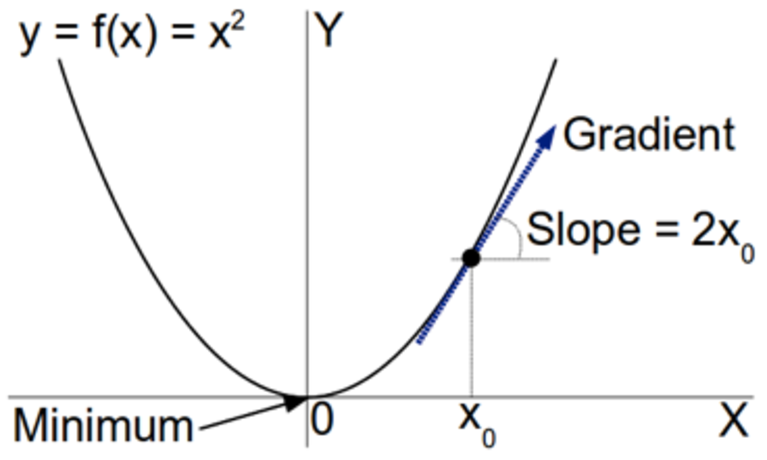
\includegraphics[width=3in]{FIGS/x_square}
\caption{The Archetypical Convex Function $f(x) = x^2$.}
\label{fig:xsquare}
\end{figure}

\begin{figure}
\centering
{\small
\begin{tabular}[t]{|l||l|}
\hline
Application & Objective \\
\hline
\hline
Least Squares & $\sum_{(u,y) \in \Omega} (x^Tu - y)^2$\\
Lasso~\cite{Tibshirani94regressionshrinkage} & $\sum_{(u,y) \in \Omega} (x^Tu - y)^2 + \mu  \|x\|_1$\\
Logisitic Regression & $\sum_{(u,y) \in \Omega} \log(1 + \exp( - y x^tu )$\\
Classification (SVM)& $\sum_{(u,y) \in \Omega} (1 - yx^{T}u)_{+}$\\
\hline
Recommendation & $\sum_{(i,j)\in\Omega} (L_i^T R_j - M_{ij})^2 + \mu\|L,R\|_F^2$\\
Labeling (CRF)~\cite{wallach:crf} & $\sum_{k} \left[ \sum_{j} x_j F_j(y_k, z_k) - \log Z(z_k) \right]$ \\
\hline
\end{tabular}}
\caption{Models currently Implemented in MADlib using the IGD-based
  approach\scriptsize In classification and regression methods, given
  a dataset $\Omega \subseteq \mathbb{R}^{N} \times \mathbb{R}$, we
  minimize the error of a predictor $x \in \mathbb{R}^N$ on a
  dataset. Given $(u,v) \in \Omega$, the methods above predict the
  value of $y$ by the equation $x^Tu$. One can add a regularization
  term to any regression or classification model, e.g., to combat
  overfitting. For example, in Lasso, we minimize the square loss
  against the data subject to an $\ell_1$ regularization.  In
  recommendation, given a matrix $M \in \mathbb{R}^{n \times m}$
  observed on a set of entries $\Omega \subseteq [n] \times [m]$, we
  fit a so called low-rank approximation, i.e., $L \in \mathbb{R}^{n
    \times k}$ and $R \in \mathbb{R}^{m \times k}$ for $k \ll
  \min\{m,n\}$ .  The low-rank matrix is regularized by the sums of the
  squares of its factors.  In Labeling with Conditional Random fields,
  we maximize the weights associated with features $(F_j)$ in the text
  predict the labels }
\label{fig:objs:grads}
\end{figure}

\paragraph*{Future Work and Challenges} We plan to work on three challenges: (1) improving performance, (2) an infrastructure to make tools in MADlib statistically robust, and (3) SAS-style Model Management. 
\begin{enumerate}
\item \textbf{Improving Performance}. IGDs are not a panacea. They
  have suboptimal runtime performance if extremely high precision is
  required. We plan to add in more both mathematical and systems-level
  optimization methods, which can be done transparently leveraging the
  decoupling provided by convex analysis.

\item \textbf{Increasing Robustness}. In its current version, MADlib
  encodes parameters of the algorithms (sometimes called
  hyperparameters) in the code itself. Some statistical techniques
  like regularization (a common technique to prevent overfitting or
  deal with poorly conditioned data) require that a user tune a
  parameter on their data. We would like to be able to expose such
  parameters in a generic way and then provide automated tuning
  techniques. In turn, our hope is to increase the robustness of these
  statistical tools automatically.

\item \textbf{Managing Models, SAS-style}. The term model management
  in the SAS literature is a distinct concept from the database
  term. The idea is to track how a model is derived, how robust its
  parameters are, which features are used in its construction. This
  has proved extremely useful in the SAS area to support higher-level
  business analytics. We plan to study this problem and develop an
  abstraction to support it.

\end{enumerate}

\subsection{Florida Contributions: Statistical Text Analytics}

%Importance of statistical text analysis 
In many domains, structured
data and unstructured text are both important assets for data
analysis. The increasing use of text analysis in enterprise
applications has increased the expectation of customers and the
opportunities for processing big data. The state-of-the-art text
analysis tools are based on statistical models and
algorithms~\cite{}. With the goal to become a framework for
statistical methods for data analysis at scale, it is important for
MADLib to include basic statistical methods to implement text analysis
tasks.

% different text analysis tasks
Basic text analysis tasks include part-of-speech (POS) tagging,
named entity extraction (NER), and entity resolution (ER)~\cite{}.
Different statistical models and algorithms are implemented for each
of these tasks with different runtime-accuracy tradeoffs. For
example, an entity resolution task could be to find all mentions in
a text corpus that refer to a real-world entity $X$. Such a task can
be done efficiently by approximate string matching~\cite{}
techniques to find all mentions in text that approximately match the
name of entity $X$. However, such a method is not as accurate as the
state-of-the-art collective entity resolution algorithms based on
statistical models, such as Conditional Random Fields
(CRFs)~\cite{crftutorial}.

% our goal
% what we've done
Based on the MADLib framework, our group set out to implement
statistical methods in SQL to support various text analysis tasks.
We use CRFs as the basic statistical model to perform more advanced
text analysis. Similar to Hidden Markov Models (HMM)~cite{}, CRF is
a leading probabilistic model for solving many text analysis tasks,
including POS, NER and ER. We implemented four different statistical
text analysis methods in MADLib, including text feature extraction,
Viterbi inference, Markov-chain Monte Carlo inference, and
approximate string matching. These statistical methods can be used
to perform different text analysis tasks as shown in Table~\ref{tab:uflmethods}.  We proceed to discuss them in turn:

\begin{table}
  \centering
\begin{tabular}{|c|c|c|c|}
  \hline
  % after \\: \hline or \cline{col1-col2} \cline{col3-col4} ...
  Statistical Methods & POS & NER & ER \\
  Text Feature Extraction & $\checkmark$ & $\checkmark$ & $\checkmark$ \\
  Viterbi Inference & $\checkmark$ & $\checkmark$ &  \\
  MCMC Inference &  & $\checkmark$ & $\checkmark$ \\
  Approximate String Matching &  &  & $\checkmark$ \\
  \hline
\end{tabular}
\label{tab:uflmethods}
\caption{Statistical Text Analysis Methods}
\end{table}

%% \dzw{Add query-driven text analysis? -- Motivation for query-driven
%% text analysis techniques for IE and ER. Compare to tasks that does
%% not need to be real-time query-driven (e.g., POS, feature
%% extraction).}

\textbf{Text Feature Extraction:} Text feature extraction is a step
in most statistical text analysis methods and it is an expensive
operation. There can be hundreds of features given a token. The main
feature types include: (1) dictionary features: whether the token
exists in each of the dictionaries; (2) regex features: whether the
token string matches various regular expressions; (3) edge features:
whether the label of the token is correlated with the label of the
previous token; (4) word features: whether the token appeared in the
training data; (5) unknown features: whether the token is unknown
from the training data; (5) start/end features: whether the token is
the first or last in the token sequence.

\textbf{Viterbi Inference:} \textit{Top-k} inference is the most
frequently used statistical method over the CRF model. Top-k inference
determines the label sequence with the top-k highest probabilities
given a token sequence %\tokenseq from a \tf \str.

The \textit{Viterbi} dynamic programming algorithm~\cite{viterbi} is
a key implementation technique for top-k inference over linear-chain
CRF models. The following equation computes the top-1 label
sequence. These can be easily extended to compute the top-k.

\vspace{-0.4cm}{\small
\begin{equation}\label{Equation:crf_viterbi}
V(i,y) = \left\{\begin{array}{lll}
    \max_{y'} (V(i-1,y') & &\\
    \quad + \sum^K_{k=1} \lambda_k f_k(y,y',x_i)), & $if$ & i\geq 0\\
    0, & $if$ & i = -1.
    \end{array}\right.
\end{equation}}

\textbf{MCMC Inference:} Markov chain Monte Carlo (MCMC) methods are
a class of randomized algorithms for estimating intractable
probability distributions over large state spaces by constructing a
Markov chain sampling process that converges to the desired
distribution. We implemented two MCMC methods in MADLib: Gibbs
sampling and Metropolis-Hastings (MCMC-MH). The iterative Gibbs
sampling algorithm is shown in Figure~\ref{Algo:Gibbs}.

\begin{figure}
\hrulefill\\
{\small
\begin{algo}{Gibbs}{N}
    w_0 \: \CALL{Init}(); w \: w_0; |  // initialize|
    \FOR{idx = 1,...,N}
        i \: idx \% n; |  // propose variable to sample next|
        w' \sim \pi (w_{i}\mid w_{-i}) |  // generate sample|
        \RETURN{| | next | | w'} |  // return a new sample|
        w \: w'; |  // update current world|
    \ENDFOR
\end{algo}}
\hrulefill\\
\caption{Pseudo-code for MCMC Gibbs sampling algorithm over a model
with $n$ variables.}  \label{Algo:Gibbs}
\end{figure}

\textbf{Approximate String Matching:} The approximate string
matching technique we use is based on qgrams~\cite{}. Qgrams---also
known as character ngrams---can be implemented efficiently inside of a
relational database. This technique as an approximate string match
was first introduced in the SQouT project~\cite{}. We used the
trigram module in PostgreSQL to create and index 3-grams over text.
Given a string ``Tim Tebow'' we can create a 3-gram by using a
sliding window of 3 characters over this text string. Given two
strings we can compare the overlap of two sets of corresponding
3-grams and compute a similarity as the approximate matching score.

%The similarity between $term_1$ and $term_2$ is computed using the
%following equation:
%
%\begin{equation}\label{}
%    S(term_1, term_2) = \frac{|term_1 \cup
%    term_2|}{min\{|term_1|,|term_2|\}}.
%\end{equation}

% main results, lessons, surprises
Statistical methods can be implemented in a relational database
efficiently. Prior work~\cite{} shows comparable performance between
in-database SQL and off-the-shelf implementations. Real-time
query-driven text analysis can be supported using indexes over a large
document corpus, which can be orders-of-magnitude faster than an
off-line batch process.

% facilities for text analysis in PostgreSQL
In the process of developing statistical methods for text analysis,
we applied and rediscovered the many PostgreSQL features for text
analysis. In addition to inverted index, user defined functions, and
user defined aggregates, we used array data types for model
parameters, trigram indexes for approximate string matching, and
recursive queries and window functions for passing states between
iterations. Also, existing modules in MADLib, such as Naive Bayes
and Sparse/Dense Matrix manipulations, can be very useful as
building blocks to implement statistical text analysis methods.

\textbf{Query-Driven Techniques}

Information Extraction (Viterbi, Feature Extraction)

Entity Resolution (MCMC, Approximate String Matching)

\textbf{Future Work}

\begin{itemize}
  \item Performance Improvement (Feature Extraction)
  \item MPP Implementation
  \item POS/IE/ER models
  \item Text Analysis query interface design
\end{itemize}
Performance Improvement (Feature Extraction) MPP Implementation
POS/IE/ER models Query-driven Text Analysis Interface (including
key-word search and more advanced)



\subsection{MADlib Futures}
\begin{itemize}
          \item Development of additional methods based on case studies in industry.  We welcome input on this front.
          \item Expand academic involvement.  Solicitation of experimental research methods from academia.  Currently lined up projects at U. Wisconsin and U. Florida (see if we can get Chris and Daisy testimonials for now; code soon.)  We welcome more collaboration with interested academics.
          \item Continued robustification of the codebase, with help from QA and engineering contributions at EMC/Greenplum on the PostgreSQL and Greenplum platforms.  We welcome offers of support from other teams to develop and maintain ports on other open-source and commercial platforms.
\end{itemize}
\section{Conclusion}



{\small \bibliographystyle{abbrv}
  \bibliography{chris.local.wopages} }

\end{document}
